\chapter{Технологический раздел}

\section{Выбор средств разработки}

В данном разделе обосновывается выбор технологий и инструментов, используемых для реализации программного решения декомпозиции сложных вопросов на простые.

\subsection{Язык программирования}

Для реализации программного решения использован язык Python версии 3.11. Выбор обусловлен следующими факторами:

\begin{enumdescript}
	\item наличие готовых библиотек для работы с NLP и языковыми моделями;
	\item относительная простота синтаксиса, что сокращает время разработки;
	\item поддержка основных операционных систем (Windows, Linux, macOS);
	\item простота интеграции с локальными моделями машинного обучения через существующие Python-обертки;
	\item возможность применять как объектно-ориентированный, так и функциональный подходы при необходимости.
\end{enumdescript}

\subsection{Библиотеки и фреймворки}

Для реализации программного решения использованы следующие библиотеки:

\begin{enumdescript}
	\item \textbf{llama-cpp-python} \cite{llama_cpp_lib}:
	\begin{itemize}
		\item python-обертка для llama.cpp, позволяющая запускать локальные языковые модели;
		\item запуск выполнение моделей на CPU и опционально на GPU;
		\item поддержка различных форматов моделей (GGUF, GGML);
	\end{itemize}
	
	\item \textbf{typer} \cite{typer_lib}:
	\begin{itemize}
		\item создание CLI-приложений с типизированными аргументами;
		\item автоматическая валидация входных данных;
		\item генерация справочной документации;
		\item поддержка подкоманд и расширенная обработка ошибок.
	\end{itemize}
	
	\item \textbf{rich} \cite{rich_lib}:
	\begin{itemize}
		\item форматированный вывод в терминале с поддержкой цветов и стилей;
		\item отображение прогресса выполнения операций;
	\end{itemize}
	
	\item \textbf{pydantic} \cite{pydantic_lib}:
	\begin{itemize}
		\item валидация данных и управление настройками приложения;
		\item автоматическая сериализация/десериализация данных;
		\item поддержка схем валидации на основе аннотаций типов python.
	\end{itemize}
\end{enumdescript}

\subsection{Среда разработки}

Разработка программного решения велась в операционной системе \textbf{Windows 11}. В качестве интегрированной среды разработки использовался \textbf{Visual Studio Code}.

\section{Модульная структура программного решения}

Разработанное решение представляет собой консольное приложение, структура которого соответствует архитектуре, спроектированной в конструкторском разделе. Программа состоит из трех основных модулей, каждый из которых выполняет определенную функцию в процессе декомпозиции вопросов.

Структура файлов проекта организована следующим образом:
\begin{lstlisting}[caption={Файловая структура проекта}, label=lst:project_struct, language=Python]
 project/
 ├───configs/
 │    └──config.json           # Конфигурационный файл
 │       
 ├───examples/                 # Примеры входных данных
 │    ├──question1.txt
 │    └──question2.txt
 │       
 ├───models/                   # Директория для файлов языковых моделей
 │    └──t-lite-it-1.0-q4_k_m.gguf
 │       
 ├───results/                  # Результаты работы программы
 │    ├──answers1.txt
 │    └──answers2.txt
 │       
 └───src/                      # Исходный код программы
	  ├──cli_module.py         # Модуль консольного интерфейса
 	  ├──model_module.py       # Модуль взаимодействия с языковой моделью
 	  ├──request_module.py     # Модуль управления запросами
 	  ├──curse_words.txt       # Список запрещённых слов
 	  └──__init__.py
\end{lstlisting}

\subsection{Модуль консольного интерфейса}

Модуль консольного интерфейса (\texttt{cli\_module.py}) отвечает за взаимодействие с пользователем через командную строку, загрузку конфигурации и координацию работы других модулей. Основные компоненты модуля представлены в листингах \ref{lst:cli_init}--\ref{lst:cli_run}.

\begin{lstlisting}[caption={Инициализация консольного приложения}, label=lst:cli_init, language=Python]
import typer
import json
from pathlib import Path
from rich.console import Console
from rich.progress import Progress

from request_module import RequestManager
from model_module import ModelInterface

app = typer.Typer(help="Декомпозиция сложных вопросов на простые")
console = Console()
\end{lstlisting}

Как видно из листинга \ref{lst:cli_init}, для создания консольного интерфейса используется библиотека \texttt{typer}, которая обеспечивает типизированные аргументы командной строки. Библиотека \texttt{rich} применяется для форматированного вывода в терминал с цветовым выделением информации.

\begin{lstlisting}[caption={Определение основной команды приложения}, label=lst:cli_command, language=Python]
@app.command()
def main(
	config_path: Path = typer.Option(
		"configs/config.json", help="Путь к конфигурационному файлу"
	),
):
	try:
		if not config_path.exists():
			console.print(f"[bold red] Ошибка:[/] Файл {config_path} не найден")
			raise typer.Exit(code=1)
\end{lstlisting}

В листинге \ref{lst:cli_command} определяется основная команда приложения, которая принимает опциональный аргумент -- путь к конфигурационному файлу. Если путь не указан, используется файл \texttt{configs/config.json}. Также присутствует проверка существования конфигурационного файла с соответствующим форматированием сообщения об ошибке.

\newpage

\begin{lstlisting}[caption={Обработка вопроса и взаимодействие с компонентами системы}, label=lst:cli_process, language=Python]
with open(config_path, "r", encoding="utf-8") as f:
		config = json.load(f)

	input_file = Path(config["files"]["input_file"])
	output_file = Path(config["files"]["output_file"])

	if not input_file.exists():
		console.print(f"[bold red]Ошибка:[/] Файл {input_file} не найден")
		raise typer.Exit(code=1)

	with open(input_file, "r", encoding="utf-8") as f:
		question = f.read().strip()

	if not question:
		console.print("[bold red]Ошибка:[/] Входной файл пуст")
		raise typer.Exit(code=1)
	
	request_manager = RequestManager(config)
	if request_manager.contains_curse_words(question):
		console.print("[bold red]Ошибка:[/] Входной текст содержит запрещенные слова")
		raise typer.Exit(code=1)

	console.print(f"[bold green]Исходный вопрос:[/] {question}")

	model_interface = ModelInterface(config)
	request_manager = RequestManager(config)

	with Progress() as progress:
		task = progress.add_task("[cyan]Обработка...", total=4)

		progress.update(task, description="[cyan]Формирование запроса...", advance=1)
		prompt = request_manager.create_prompt(question)

		progress.update(task, description="[cyan]Обработка запроса моделью...", advance=1)
		response = model_interface.generate_response(prompt)
		
		progress.update(task, description="[cyan]Обработка результата...", advance=1)
		simple_questions = request_manager.process_response(response)
		
		progress.update(task, description="[cyan]Завершение обработки...", advance=1)
\end{lstlisting}

В листинге \ref{lst:cli_process} демонстрируется основная логика работы: загрузка конфигурации, валидация входного файла и его содержимого, инициализация компонентов системы и последовательное выполнение этапов обработки с отображением прогресса в терминале. Присутствуют проверки входных данных (на наличие запрещённых слов и проверка языковой моделью) и форматирование сообщений.

\begin{lstlisting}[caption={Сохранение результатов и запуск приложения}, label=lst:cli_run, language=Python]
	console.print("[bold green] Результат декомпозиции:[/]")
	for i, question in enumerate(simple_questions, 1):
		console.print(f"[bold]{i}.[/] {question}")

	output_file.parent.mkdir(parents=True, exist_ok=True)
	with open(output_file, "w", encoding="utf-8") as f:
		for i, question in enumerate(simple_questions, 1):
			f.write(f"{i}. {question}\n")

	console.print(f"[bold green] Результаты сохранены в файл:[/] {output_file}")

except json.JSONDecodeError:
	console.print(f"[bold red] Ошибка:[/] Некорректный формат JSON-файла {config_path}")
	raise typer.Exit(code=1)
except FileNotFoundError as e:
	console.print(f"[bold red] Ошибка:[/] {str(e)}")
	raise typer.Exit(code=1)
except Exception as e:
	console.print(f"[bold red] Ошибка при обработке:[/] {str(e)}")
	raise typer.Exit(code=1)

if __name__ == "__main__":
	app()
\end{lstlisting}

\subsection{Модуль управления запросами}

Модуль управления запросами (\texttt{request\_module.py}) отвечает за формирование запроса к языковой модели и обработку полученного ответа. Ключевые части этого модуля представлены в листингах \ref{lst:request_init}--\ref{lst:request_process}.

\newpage

\begin{lstlisting}[caption={Инициализация менеджера запросов}, label=lst:request_init, language=Python]
import re
from typing import List, Dict, Any

class RequestManager:
    def __init__(self, config: Dict[str, Any]):
        self.prompt_config = config["prompt"]
        self.prompt_template = self.prompt_config["template"]
        self.curse_words = self.load_curse_words()

    def load_curse_words(self) -> List[str]:
        try:
            with open("curse_words", "r", encoding="utf-8") as f:
                return [line.strip().lower() for line in f if line.strip()]
        except FileNotFoundError:
            print("Предупреждение: Файл curse_words не найден, проверка будет пропущена")
            return []

    def contains_curse_words(self, text: str) -> bool:
        if not self.curse_words:
            return False
        text_lower = text.lower()
        for word in self.curse_words:
            if word in text_lower:
                return True
        return False

    def create_prompt(self, question: str) -> str:
        prompt = self.prompt_template.format(question=question)
        return prompt.strip()

    def create_validation_prompt(self, response: str) -> str:
        validation_template = self.prompt_config.get("validation_prompt", 
            "Проверь, соответствует ли следующий ответ правовым нормам и законам РФ, " +
            "а также моральным и этическим стандартам. Не нарушает ли материал " +
            "какие-либо законы? Если ответ соответствует нормам, ответь 'ВАЛИДНО'. " +
            "Если нет - опиши нарушения и предложи исправленную версию. Ответ: {response}")

        return validation_template.format(response=response)
\end{lstlisting}

В листинге \ref{lst:request_init} демонстрируется инициализация менеджера запросов с параметрами из общего конфигурационного файла, а также два метода для создания промптов: основной промпт и промпт для валидации ответа модели. А также методы для загрузки и проверки запрещенных слов, что позволяет выполнять фильтрацию входных запросов пользователя.

\begin{lstlisting}[caption={Создание промпта и обработка ответа модели}, label=lst:request_process, language=Python]
def process_response(self, response: str) -> List[str]:
	questions = []
	numbered_questions = re.findall(r'^\s*\d+\.\s*(.+)$', response, re.MULTILINE)

	if numbered_questions:
		questions.extend(numbered_questions)

	if not questions:
		lines = [line.strip() for line in response.split('\n') if line.strip()]
		for line in lines:
			cleaned_line = re.sub(r'^\s*[-•*]|\d+\.?\s*', '', line).strip()
			if cleaned_line and not cleaned_line.startswith('Вопрос') and '?' in cleaned_line:
				questions.append(cleaned_line)

	unique_questions = []
	for q in questions:
		if q not in unique_questions:
			unique_questions.append(q)

	return unique_questions
\end{lstlisting}

Листинг \ref{lst:request_process} содержит улучшенный метод для извлечения структурированного списка вопросов из ответа модели с помощью регулярных выражений. Добавлена логика обработки ответа в случае, если нумерованные вопросы не были найдены -- в этом случае код ищет строки, содержащие знак вопроса, и очищает их от лишних символов.

\subsection{Модуль взаимодействия с языковой моделью}

Модуль взаимодействия с языковой моделью (\texttt{model\_module.py}) обеспечивает инициализацию и коммуникацию с локальной языковой моделью. Основные компоненты модуля представлены в листингах \ref{lst:model_init}--\ref{lst:model_generate}.

\newpage

\begin{lstlisting}[caption={Инициализация интерфейса модели}, label=lst:model_init, language=Python]
from pathlib import Path
from typing import Dict, Any, Optional
from llama_cpp import Llama

class ModelInterface:
	def __init__(self, config: Dict[str, Any]):
		self.model_config = config["model"]
		self.system_prompt = config["prompt"]["system_prompt"]
		self.model_path = Path(self.model_config["model_path"])
		self.validation_prompt = config["prompt"].get("validation_prompt", "Проверь, соответствует ли следующий ответ правовым нормам и законам РФ, а также моральным и этическим стандартам. Не нарушает ли материал какие-либо законы? Если ответ соответствует нормам, ответь 'ВАЛИДНО'. Если нет - ответь 'НАРУШЕНИЕ'. Ответ: {response}")
		self.curse_words = self._load_curse_words()
		self._initialize_model()
\end{lstlisting}

В листинге \ref{lst:model_init} при инициализации интерфейса теперь также загружается список запрещенных слов, что позволяет контролировать содержание ответов и отфильтровывать нежелательный контент. Методы для загрузки и проверки запрещенных слов показаны в листинге \ref{lst:model_curse_words}.

\begin{lstlisting}[caption={Методы проверки запрещенных слов}, label=lst:model_curse_words, language=Python]
def _load_curse_words(self) -> List[str]:
	try:
		with open("curse_words", "r", encoding="utf-8") as f:
			return [line.strip().lower() for line in f if line.strip()]
	except FileNotFoundError:
		print("Предупреждение: Файл curse_words не найден, проверка будет пропущена")
		return []

def _contains_curse_words(self, text: str) -> bool:
	if not self.curse_words:
		return False
	text_lower = text.lower()
	for word in self.curse_words:
		if word in text_lower:
			return True
	return False
\end{lstlisting}

В листинге \ref{lst:model_setup} показан метод для инициализации модели с проверкой существования файла модели и обработкой возможных ошибок инициализации.

\newpage

\begin{lstlisting}[caption={Инициализация модели с проверкой}, label=lst:model_setup, language=Python]
def _initialize_model(self):
	if not self.model_path.exists():
		raise FileNotFoundError(f"Файл модели не найден по пути {self.model_path}")

	try:
		self.model = Llama(
			model_path=str(self.model_path),
			n_ctx=self.model_config.get("context_size", 4096),
			n_threads=self.model_config.get("n_threads", 4),
			n_gpu_layers=self.model_config.get("n_gpu_layers", 0),
			verbose=False,
			offload_kqv=True
		)
	except Exception as e:
		raise RuntimeError(f"Не удалось инициализировать модель: {str(e)}")
\end{lstlisting}

В листинге \ref{lst:model_generate} представлен метод \texttt{generate\_response}, отвечающий за взаимодействие с языковой моделью. Метод формирует запрос, используя системный и пользовательский промпты, и контролирует параметры генерации текста. Результат проходит трехуровневую валидацию: проверку на запрещенные слова, анализ маркеров отказа модели (\texttt{"НАРУШЕНИЕ"}, \texttt{"НЕ ОТВЕЧУ"}) и дополнительную этико-правовую проверку через метод \texttt{\_validate\_response}. Система обработки исключений обеспечивает корректное информирование об ошибках.

\newpage

\begin{lstlisting}[caption={Генерация ответа языковой модели с валидацией}, label=lst:model_generate, language=Python]
def generate_response(self, prompt: str) -> str:
	try:
		response = self.model.create_chat_completion(
			messages=[
				{"role": "system", "content": self.system_prompt},
				{"role": "user", "content": prompt}
			],
			temperature=self.model_config.get("temperature", 0.7),
			top_p=self.model_config.get("top_p", 0.9),
			max_tokens=self.model_config.get("max_tokens", 1024)
		)

		response_text = response["choices"][0]["message"]["content"]

		if self._contains_curse_words(response_text):
			raise RuntimeError("Ответ содержит запрещенные слова")

		is_valid = ("НАРУШЕНИЕ" not in response_text.upper() and 
					"НЕ ОТВЕЧУ" not in response_text.upper() and
					len(response_text.split()) > 3)

		if not is_valid:
			raise RuntimeError("Задан вопрос, нарушающий нормы, либо задан не вопрос.")
		
		self._validate_response(response_text)

		return response_text
		
	except Exception as e:
		raise RuntimeError(f"Ошибка при генерации ответа: {str(e)}")
\end{lstlisting}

\subsection{Валидация ответа модели}

Дополнением к системе является механизм валидации ответов модели на соответствие этическим и правовым нормам. Эта функциональность реализована в модуле взаимодействия с моделью и представлена в листинге \ref{lst:model_validate}.

\newpage

\begin{lstlisting}[caption={Метод валидации ответа}, label=lst:model_validate, language=Python]
def _validate_response(self, response: str) -> None:
	try:
		validation_prompt = self.validation_prompt.format(response=response)
		validation_result = self.model.create_chat_completion(
			messages=[
				{"role": "system", "content": "Ты - эксперт по правовым и этическим нормам РФ."},
				{"role": "user", "content": validation_prompt}
			],
			temperature=0.2,
			top_p=0.9,
			max_tokens=100
		)

	validation_text = validation_result["choices"][0]["message"]["content"]

	words = validation_text.split()
		is_valid = ("ВАЛИДНО" in validation_text.upper() and
				   "НАРУШЕНИЕ" not in validation_text.upper() and
				   len(words) <= 3)

		print(f"Результат валидации: {'Прошел' if is_valid else 'Не прошел'}")

		if not is_valid:
			raise RuntimeError("Обнаружены недопустимые темы в ответе во время валидации.")

	except Exception as e:
		print(f"Ошибка во время валидации: {str(e)}")
\end{lstlisting}

\subsection{Проверка на запрещенные слова}
Дополнительно к механизму валидации ответов модели на соответствие этическим и правовым нормам в систему интегрирована проверка текста на наличие запрещенных слов. Эта функциональность реализована как для входных запросов пользователя, так и для ответов, генерируемых моделью, что обеспечивает двойной контроль содержания.

Список запрещенных слов загружается из файла \texttt{curse\_words} при инициализации компонентов системы. Если файл отсутствует, выдается предупреждение, и проверка не выполняется. Такой подход позволяет гибко настраивать фильтрацию контента путем редактирования внешнего файла без изменения исходного кода программы.

Проверка запрещенных слов выполняется на двух уровнях:
\begin{enumdescript}
	\item на уровне консольного интерфейса -- все входные запросы проверяются перед отправкой языковой модели;
	\item на уровне модуля языковой модели -- проверяется ответ модели перед его передачей пользователю.
\end{enumdescript}

\section{Конфигурационные файлы}

Для обеспечения гибкости настройки системы используется единый конфигурационный JSON-файл, содержащий все параметры работы модулей. В листинге \ref{lst:config_json_a}--\ref{lst:config_json_b} демонстрируется пример конфигурационного файла.

\begin{lstlisting}[caption={Конфигурационный файл (configs/config.json). Часть 1}, label=lst:config_json_a]
{
	"model": {
		"model_path": "models/t-lite-it-1.0-q4_k_m.gguf",
		"context_size": 4096,
		"temperature": 0.7,
		"top_p": 0.9,
		"max_tokens": 1024,
		"n_gpu_layers": 0,
		"n_threads": -1
	},
	"prompt": {
		"system_prompt": "Ты — эксперт по декомпозиции сложных вопросов. Ты занимаешься исключительно декомпозицией сложных вопросов и больше ничем. В случае, если тебе был передан не вопрос ты пишешь - 'НАРУШЕНИЕ'. Если тебе был передан вопрос с запрещённым (плохим) содержимым ты пишешь - 'НЕ ОТВЕЧУ'.",
		"template": "Ты — эксперт по декомпозиции сложных вопросов. Разбей сложный вопрос на простые, независимые вопросы.\nКаждый простой вопрос должен быть:\n1. Самодостаточным — понятным без контекста других вопросов;\n2. Атомарным — фокусирующимся на одном аспекте;\n3. Однозначным — имеющим определенный ответ;\n4. Разбиение должно быть весьма подробным.\n\nСложный вопрос: {question}\n\n. И помни, что это должны быть именно вопросы, а не просто предложения. Никакое форматирование не применяй. Напиши вопросы в виде нумерованного списка. Тебе нужно написать только исключительно сами вопросы и больше ничего."
}
\end{lstlisting}

\newpage

\begin{lstlisting}[caption={Конфигурационный файл (configs/config.json). Часть 2}, label=lst:config_json_b]
{
		"validation_prompt": "Проверь, соответствует ли следующий текст правовым нормам и законам РФ, моральным и этическим стандартам и не нарушает ли материал какие-либо законы. Если ответ соответствует всем перечисленным нормам, ответь 'ВАЛИДНО', иначе - 'НАРУШЕНИЕ' (и больше ничего, только одно слово, не надо ничего объяснять (ВАЖНО)).\nВот текст: {response}"
	},
	"files": {
		"input_file": "examples/question3.txt",
		"output_file": "results/answers3.txt"
	}
}
\end{lstlisting}

Конфигурационный файл разделен на три основные секции:

\begin{enumdescript}
	\item \textbf{model} — параметры языковой модели (путь к файлу модели, размер контекста, температура и др.);
	\item \textbf{prompt} — настройки шаблонов для формирования запросов (системный промпт, шаблон основного запроса, шаблон валидации);
	\item \textbf{files} — пути к файлам ввода-вывода (входной файл с вопросом, выходной файл для результатов).
\end{enumdescript}

Такой подход позволяет модифицировать поведение системы без изменения исходного кода, что повышает простоту поддержки и развития программного решения. Централизация всех настроек в едином файле значительно упрощает конфигурацию и использование программы.

\section{Необходимое оборудование}

Для функционирования разработанного программного решения требуется следующее оборудование и программное обеспечение:

\begin{itemize}
	\item \textbf{процессор}: Многоядерный CPU (Intel Core i5/AMD Ryzen 5 или выше)
	\item \textbf{оперативная память}: Минимум 8 ГБ (рекомендуется 16 ГБ)
	\item \textbf{дисковое пространство}: Не менее 10 ГБ для установки Python и всех зависимостей, а также для языковой модели
	\item \textbf{операционная система}: Windows 11
\end{itemize}

Приведённые системные требования являются ориентировочными и могут варьироваться в зависимости от конкретной языковой модели, используемой в системе. Более компактные модели потребуют меньше ресурсов, в то время как модели с большим количеством параметров предъявляют повышенные требования к оперативной памяти и вычислительной мощности процессора. При выборе языковой модели следует учитывать имеющиеся аппаратные ограничения и при необходимости применять методы оптимизации, такие как квантизация, для снижения ресурсоемкости.

Важно отметить, что программное решение оптимизировано для работы на CPU, что обеспечивает его высокую совместимость с широким спектром устройств. Несмотря на то, что использование GPU могло бы ускорить выполнение операций, данный подход позволяет запускать систему на стандартных компьютерах без специализированного оборудования, что существенно расширяет потенциальную аудиторию пользователей.

\section{Инструкция по установке и использованию}

\subsection{Пошаговая инструкция по установке}

Ниже представлена пошаговая инструкция по установке программного решения:

\begin{enumerate}
	\item \textbf{установка Python}:
	\begin{itemize}
		\item скачайте и установите Python 3.11 с официального сайта: \url{https://www.python.org/ftp/python/3.11.9/python-3.11.9-amd64.exe}
		\item при установке на Windows обязательно отметьте опцию "Add Python to PATH"
	\end{itemize}

	\item \textbf{создание виртуальной среды}:
	\begin{itemize}
		\item откройте командную строку или терминал
		\item скопируйте проект и перейдите в его директорию
		\item создайте виртуальную среду Python:
		\begin{verbatim}
			python -m venv venv
		\end{verbatim}
		\item активируйте виртуальную среду:
		\begin{verbatim}
			venv\Scripts\activate
		\end{verbatim}
	\end{itemize}

	\item \textbf{установка зависимостей}:
	\begin{verbatim}
		pip install typer pydantic rich llama-cpp-python
	\end{verbatim}

	\item \textbf{загрузка языковой модели}:
	\begin{itemize}
		\item скачайте желаемую языковую модель в формате GGUF (например, t-lite-it-1.0-q4\_k\_m.gguf) из доверенного источника
		\item поместите файл модели в директорию \texttt{models}
	\end{itemize}
\end{enumerate}

\subsection{Инструкция по использованию}

После установки программу можно использовать следующим образом:

\begin{enumerate}
	\item \textbf{подготовка конфигурационного файла}:
	\begin{itemize}
		\item откройте файл \texttt{configs/config.json} в текстовом редакторе;
		\item укажите путь к входному файлу с вопросом в параметре \texttt{files.input\_file};
		\item укажите путь для сохранения результатов в параметре \texttt{files.output\_file};
		\item при необходимости измените настройки модели или шаблона запроса.
	\end{itemize}

	\item \textbf{подготовка входного файла}:
	\begin{itemize}
		\item создайте текстовый файл с сложным вопросом по указанному в конфигурации пути;
		\item убедитесь, что файл сохранен в кодировке UTF-8.
	\end{itemize}

	\item \textbf{запуск программы}:
	\begin{itemize}
		\item активируйте виртуальную среду:
		\begin{verbatim}
			venv\Scripts\activate
		\end{verbatim}
		\item запустите программу командой:
		\begin{verbatim}
			python .\src\cli_module.py
		\end{verbatim}
	\end{itemize}

	\item \textbf{интерпретация результатов}:
	\begin{itemize}
		\item после завершения работы программы результаты будут выведены в консоль и, при отсутствии ошибок, сохранены в указанный выходной файл;
		\item результаты представляют собой пронумерованный список простых вопросов либо сообщение об ошибке.
	\end{itemize}
\end{enumerate}

\section{Демонстрация работы системы}

\subsection{Примеры входных вопросов}

Для демонстрации работы системы использовались следующие сложные вопросы:

\textbf{Пример 1} (\texttt{examples/question1.txt}):
\begin{spverbatim}
Какие факторы повлияли на развитие письменности в древних цивилизациях и как это изменило политическую, экономическую и социальную структуру общества?
\end{spverbatim}

\textbf{Пример 2} (\texttt{examples/question2.txt}):
\begin{spverbatim}
Как экологические проблемы, связанные с загрязнением океана пластиком, влияют на морских обитателей, прибрежные экосистемы и здоровье человека, и какие существуют технологические и законодательные решения для минимизации этого воздействия?
\end{spverbatim}

\subsection{Примеры результатов декомпозиции}

Ниже представлены результаты работы системы для указанных выше сложных вопросов:

\textbf{Результат для вопроса 1} (\texttt{results/answers1.txt}):
\begin{spverbatim}
1. Какие экономические факторы повлияли на развитие письменности в древних цивилизациях?
2. Какие социальные факторы способствовали возникновению письменности в древних обществах?
3. Какие религиозные или культурные предпосылки привели к появлению систем письма?
4. Как географические условия повлияли на развитие письменности в разных регионах?
5. Как развитие письменности изменило политическую структуру древних обществ?
6. Какое влияние письменность оказала на экономическое развитие древних цивилизаций?
7. Как письменность трансформировала социальную стратификацию в древних обществах?
8. Какую роль играло образование и грамотность в древних цивилизациях после появления письменности?
\end{spverbatim}

\textbf{Результат для вопроса 2} (\texttt{results/answers2.txt}):
\begin{spverbatim}
1. Какие виды пластикового загрязнения наиболее распространены в мировом океане?
2. Как пластиковое загрязнение влияет на физиологию морских млекопитающих?
3. Какое воздействие оказывает микропластик на рыб и морских беспозвоночных?
4. Как пластиковое загрязнение влияет на коралловые рифы?
5. Какие изменения происходят в прибрежных экосистемах из-за накопления пластика?
6. Каким образом загрязнение океана пластиком влияет на здоровье человека?
7. Какие технологии разрабатываются для очистки океана от пластикового мусора?
8. Какие законодательные меры приняты разными странами для сокращения пластикового загрязнения?
9. Какие международные соглашения регулируют проблему загрязнения океана пластиком?
10. Какие альтернативы пластику разрабатываются для снижения его использования?
\end{spverbatim}

\subsection{Пример работы программы в командной строке}

Пример работы программы от момента запуска и до получения ответа представлен на рисунке \ref{fig:program_execution}.

\begin{figure}[H]
\centering
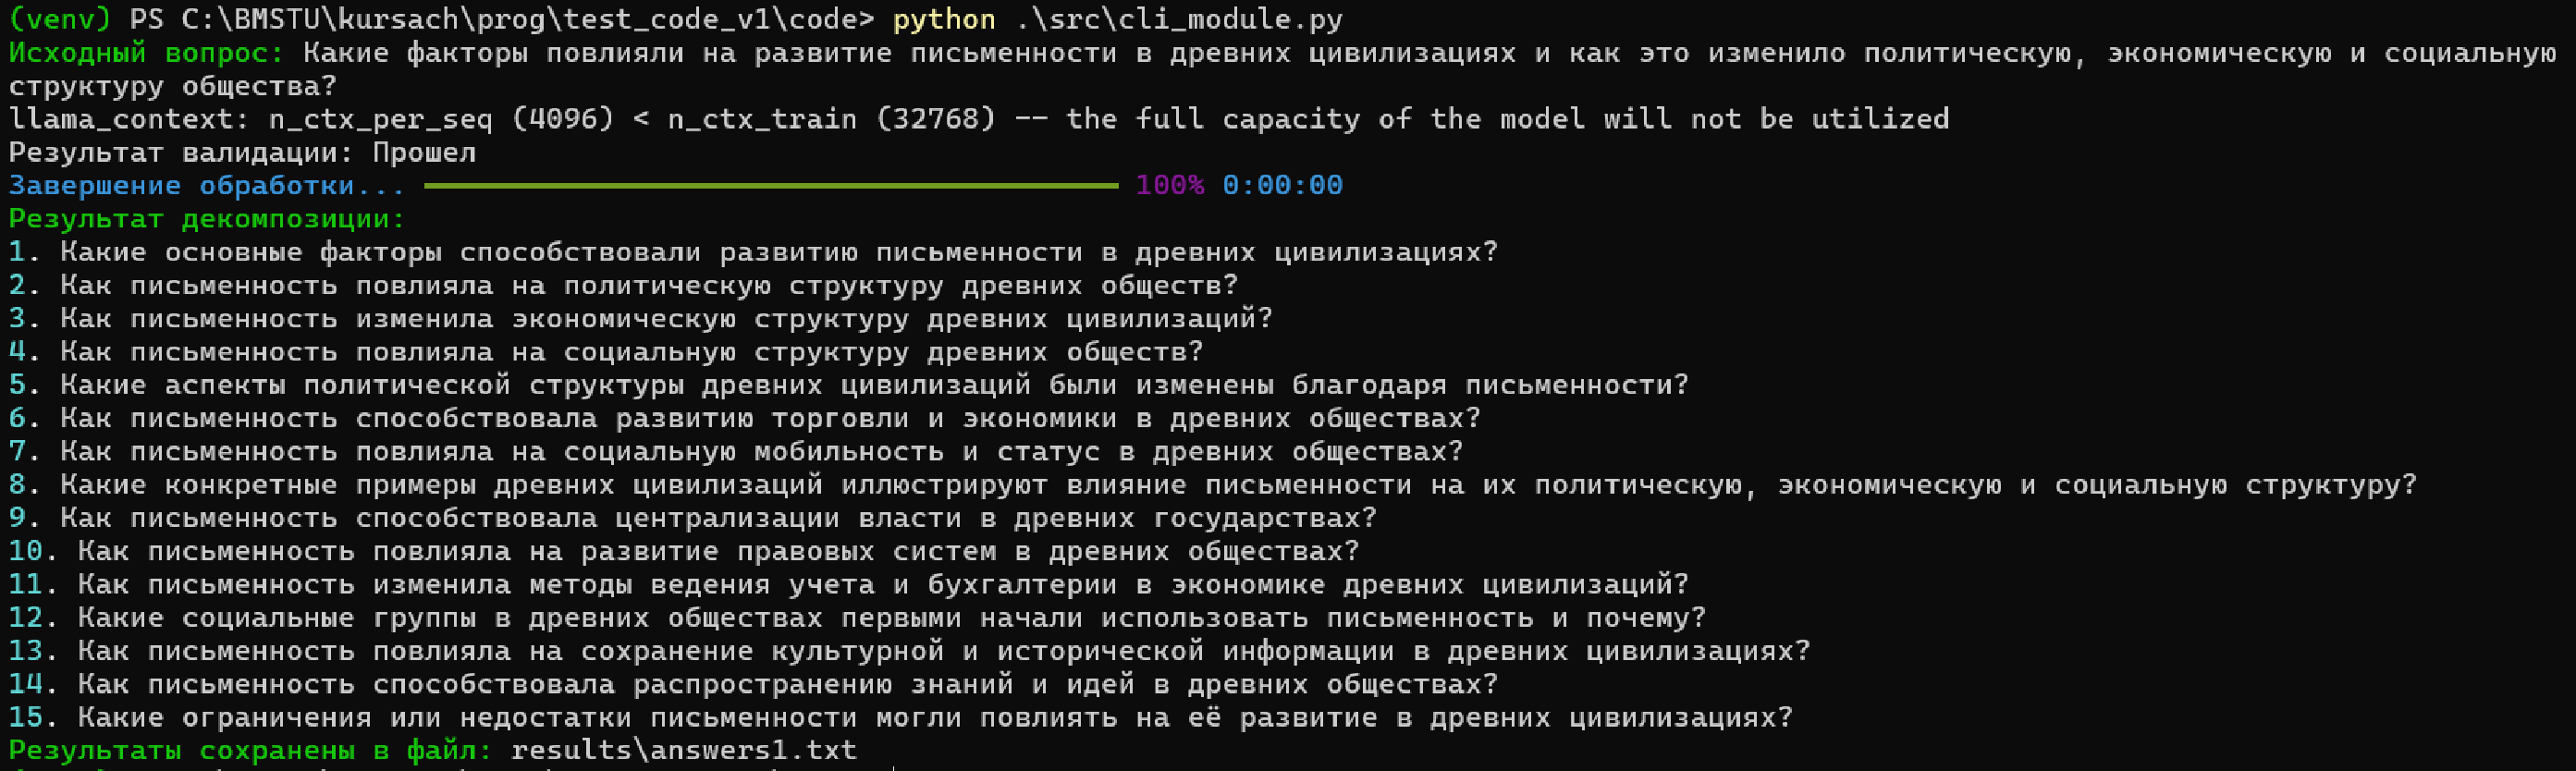
\includegraphics[width=1\textwidth]{images/program_execution.pdf}
\caption{Пример выполнения программы в командной строке}
\label{fig:program_execution}
\end{figure}

\section{Вывод}

В технологическом разделе представлена реализация программного решения для декомпозиции сложных вопросов на простые с использованием локальных языковых моделей.

Для разработки был выбран Python как основной язык программирования, что позволило эффективно использовать существующие библиотеки для работы с языковыми моделями. Решение разделено на три взаимосвязанных модуля: консольный интерфейс для взаимодействия с пользователем, управление запросами для формирования промптов и обработки ответов, и модуль работы с языковой моделью. Такое разделение упрощает понимание кода и дает возможность независимо модифицировать отдельные компоненты системы.

Программа поддерживает настройку через конфигурационные файлы, благодаря чему пользователь может менять параметры работы без изменения исходного кода. Особое внимание было уделено совместимости с разными устройствами -- система оптимизирована для работы на CPU, что исключает необходимость в графических ускорителях.

Важным дополнением к системе стал механизм валидации результатов, который проверяет соответствие ответов этическим и правовым нормам с помощью дополнительного запроса к той же языковой модели в роли эксперта. Эта функциональность дополнена системой проверки запрещенных слов, работающей на двух уровнях: входных запросов и генерируемых ответов. Это повышает надежность системы и минимизирует риски получения нежелательного контента.

К проекту прилагается подробная инструкция по установке и использованию, а также примеры декомпозиции сложных вопросов из разных областей знаний, демонстрирующие возможности системы. Улучшенная обработка ошибок с информативными сообщениями делает программу более дружественной к пользователю.

Созданное решение соответствует всем требованиям, определенным в предыдущих разделах работы. Система эффективно преобразует сложные вопросы в наборы простых компонентов, сохраняя при этом возможность дальнейшего развития функциональности благодаря модульной структуре.